\chapter{Results} \label{chap:results}
Main purpose of the thesis is the implementation of a navigation system that uses measurements from different sensors, fuses the sensory data together in order to make presumably better quality estimate of the position and the orientation of the underwater robot. Existing data from the real missions were used to carry out the initial trials. It is useful to mention that there is no exact ground truth for underwater robot localization available. GPS signal, if available, could serve as an absolute position reference: either directly or in form of LBL. Experimental results have been obtained for different missions. Good news, however, is that the absolute depth measurement is quite accurate and frequent, making AUV localisation a 2D task.  

\section{Real navigation scenario} \label{sec:real-scenario}
Authentic data taken from previously recorded Nessie mission were used to simulate the algorithm ``offline'' as the part of the stage intended for testing and correcting. Besides, being able to repeat the same measurement scenario enables more insight in filtering process and benefits of fusing together the sensor data. \textit{.bag} files (\url{http://www.ros.org/wiki/}) containing recorded real-time messages with sensor measurements, were used as source. Furthermore, it allows designing the code in its original C++ form that will require little modification once deployed on the vehicle in form of ROS package since \textit{.bag} files emulate authentic messages and timestamps. One of the deficiencies of the evaluation of localisation results is the fact that there is no exact ground truth to compare the result with. Dead reckoning localisation substituted with occasional LBL position updates was compared with the localisation obtained after filtering (Figures ~\ref{fig:auv-sim-straight2}, ~\ref{fig:auv-sim-straight1}) for the recorded straight line trajectory mission. 

\T{Selecting a heading measurement with good performance}
For a high-end underwater vehicle such as Nessie, supplied with FOG-based INS, DVL and LBL, main source of navigation error is influenced by transformation of vehicle-referenced velocities to world-referenced velocities \cite{bahr08}, particularly due to yaw (heading) measurement errors. Yaw can be measured using several devices, each having different accuracy and performance. Simulation with data from previous missions was carried out to see which device gives the best performance for a given underwater vehicle. 

Heading calculated by integrating FOG's yaw rate - tends to be accurate and fast, less prone to noise. Nevertheless, it is calculated each time by appending yaw rate value integrated in time on the previous yaw value (relative measurement). Therefore, it is sensible on initial absolute heading measurement. In case initial yaw is imprecise, a constant bias exists in yaw measurement (Figure ~\ref{fig:auv-sim-straight1}). Constant bias causes sudden steps in position estimate obtained using EKF. This is expected scenario since the sensor responsible for measuring initial heading is magnetic compass, device sensitive to disturbances coming from environment (Figure ~\ref{fig:magnetic-disturb}). In real experiments biggest obstacle was proper calibration of magnetic compass. In practice, tests have showed many failures in compass heading measurement, possibly due to calibration and magnetic declination. There is yet space to do more testing with better compass tuning. To overcome the problem of accurate yaw measurement, EKF used in experiments will either ignore the yaw measurement (it is possible since sensor fusion successfully compensates missing heading information with yaw rate obtained from FOG) or use it with high variance assigned to yaw measurement. 
%Finally, initial heading is given with magnetic compass.

\T{Loch Earn dataset - straight line movement}: Example of basic EKF localisation using inertial measurements aided with LBL acoustic positioning system was tested on straight line movement of approximately 80 m length, recorded at the lake Loch Earn. For simulation purposes, sensor measurements are stored in a \textit{.bag} file, that can be replayed, producing real-time messages of sensor measurements as they originally occurred. At this point, it is important to revise which sensors were used, their main features and, finally, filtering parameters. 

Standard sensor configuration comprising of pressure sensor, magnetic compass, FOG and DVL is used in the mission. Absolute position correction was carried out using LBL system. Important fact is that the heading was measured with magnetic compass only at the beginning. Later on, it kept being calculated by integrating yaw rate obtained from FOG. Alternative solution for the heading measurement would be the usage of compass for direct acquiring of yaw, but such option exposed calibration difficulties. Result of EKF localisation algorithm was shown in north-east map (Figure ~\ref{fig:sim-straight2}, ~\ref{fig:sim-straight1}). Different parameter values for EKF were tested. Table ~\ref{tab:ekf-params} revises all filter parameters used for filter tuning, together with their role. Essentially, setting high standard deviation for a Gaussian of a certain parameter can be interpreted as having more uncertainty in value that it represents - whether it is a measurement uncertainty or uncertainty of the predicted value (model uncertainty). Therefore, we can choose to be confident in certain sensor measurement and/or certain model prediction, and observe the simulation outcome of such setting. Setting the parameters properly improves the performance of the filter.  
\addtocounter{footnote}{1}
\footnotetext[\value{footnote}]{as it appears in algorithm equations}  
\begin{table*}
\centering
	\caption{EKF navigation parameters.}
	\label{tab:ekf-params}
\begin{tabular}{llll}
\toprule
Parameter      &     Signature $^{\decimal{footnote}}$     &     Units     &    Description  \\
\midrule
                         & \multicolumn{3}{c}{standard deviation of the ... } \\ 
\multirow{1}{*}{SDNorth} & \multirow{1}{*}{$\sigma_{n}$} & \multirow{1}{*}{$m$} & \multirow{1}{*}{north observation} \\
\multirow{1}{*}{SDEast}  & \multirow{1}{*}{$\sigma_{e}$} & \multirow{1}{*}{$m$} & \multirow{1}{*}{east observation} \\
\multirow{1}{*}{SDDepth} & \multirow{1}{*}{$\sigma_{d}$} & \multirow{1}{*}{$m$} & \multirow{1}{*}{depth observation} \\
\multirow{1}{*}{SDAltitude} & \multirow{1}{*}{$\sigma_{a}$} & \multirow{1}{*}{$m$} & \multirow{1}{*}{altitude observation} \\
\multirow{1}{*}{SDu} & \multirow{1}{*}{$\sigma_{u}$} & \multirow{1}{*}{$\frac{m}{s}$} & \multirow{1}{*}{surge velocity observation} \\
\multirow{1}{*}{SDv} & \multirow{1}{*}{$\sigma_{v}$} & \multirow{1}{*}{$\frac{m}{s}$} & \multirow{1}{*}{sway velocity observation} \\
\multirow{1}{*}{SDw} & \multirow{1}{*}{$\sigma_{w}$} & \multirow{1}{*}{$\frac{m}{s}$} & \multirow{1}{*}{heave velocity observation} \\
\multirow{1}{*}{SDyaw} & \multirow{1}{*}{$\sigma_{\psi}$} & \multirow{1}{*}{$rad$} & \multirow{1}{*}{heading observation} \\
\multirow{1}{*}{SDpitch} & \multirow{1}{*}{$\sigma_{\varphi}$} & \multirow{1}{*}{$rad$} & \multirow{1}{*}{pitch observation} \\
\multirow{1}{*}{SDyawRate} & \multirow{1}{*}{$\sigma_{\dot{\psi}}$} & \multirow{1}{*}{$\frac{rad}{s}$} & \multirow{1}{*}{heading rate observation} \\
\multirow{1}{*}{SDpitchRate} & \multirow{1}{*}{$\sigma_{\dot{\varphi}}$} & \multirow{1}{*}{$\frac{rad}{s}$} & \multirow{1}{*}{pitch rate observation} \\
\midrule
                         & \multicolumn{3}{c}{standard deviation of the ... process noise} \\
\multirow{1}{*}{SDuModel} & \multirow{1}{*}{$\sigma_{\dot{u}}$}  & \multirow{1}{*}{$\frac{m}{s^{2}}$} & \multirow{1}{*}{surge acceleration} \\
\multirow{1}{*}{SDvModel} & \multirow{1}{*}{$\sigma_{\dot{v}}$}  & \multirow{1}{*}{$\frac{m}{s^{2}}$} & \multirow{1}{*}{sway acceleration} \\
\multirow{1}{*}{SDwModel} & \multirow{1}{*}{$\sigma_{\dot{w}}$}  & \multirow{1}{*}{$\frac{m}{s^{2}}$} & \multirow{1}{*}{heave acceleration} \\
\multirow{1}{*}{SDyawRateModel} & \multirow{1}{*}{$\sigma_{\dot{v}}$}  & \multirow{1}{*}{$\frac{rad}{s^{2}}$} & \multirow{1}{*}{yaw acceleration} \\
\multirow{1}{*}{SDpitchRateModel} & \multirow{1}{*}{$\sigma_{\dot{w}}$}  & \multirow{1}{*}{$\frac{rad}{s^{2}}$} & \multirow{1}{*}{pitch acceleration} \\
\bottomrule
\end{tabular} 
\end{table*}
Straight line movement with authentic sensor measurements recorded in Loch Earn was a basis for initial tests of the EKF localisation algorithm. Red line shows the dead reckoning navigation, which is directly updated with absolute position update (LBL). Dead reckoning uses values periodically ($\approx$5$Hz$) obtained from DVL and FOG (linear velocities: $u$ and $v$ and heading $\psi$, respectfully), and substitutes them into equations similar to ones used for north and east prediction within prediction model: 
$$ north = north + (uT+\dot{u}\frac{T^{2}}{2})\cos(\psi) - (vT+\dot{v}\frac{T^{2}}{2})\sin(\psi) $$
$$ east  = east  + (uT+\dot{u}\frac{T^{2}}{2})\sin(\psi) + (vT+\dot{v}\frac{T^{2}}{2})\cos(\psi) $$
% SDnorth/east = 5 $cm$, 
% SDnorth/east = 5 $cm$, 
\begin{figure}%[htb]
  \centering
    \subfigure[N/E localisation. Yaw was calculated by integrating yaw rate periodically measured using FOG.] {\label{fig:sim-straight2}
	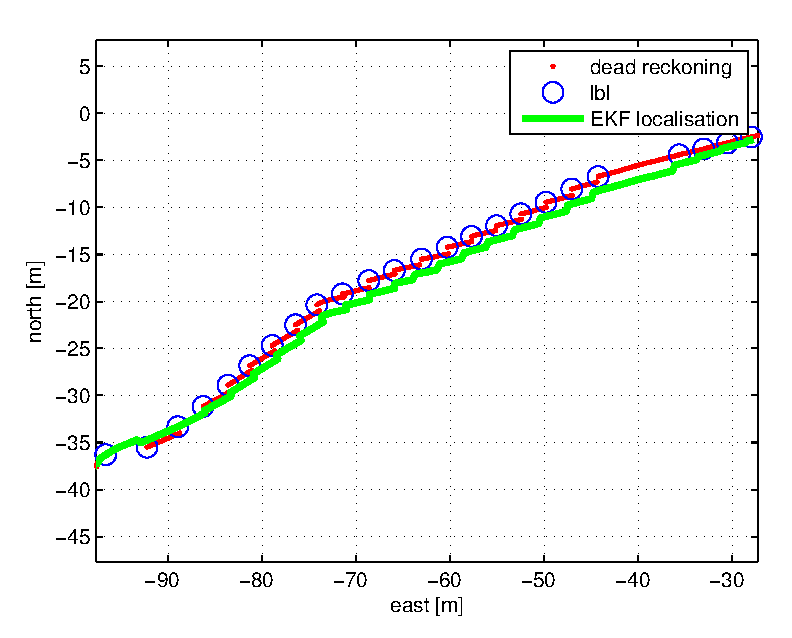
\includegraphics[width=0.48\linewidth]{simulations/fig/sim-straight2.eps}}
    \subfigure[Heading estimation. Biased yaw measurement not being corrected due to high confidence in yaw measurement.] {\label{fig:yaw-straight2}
    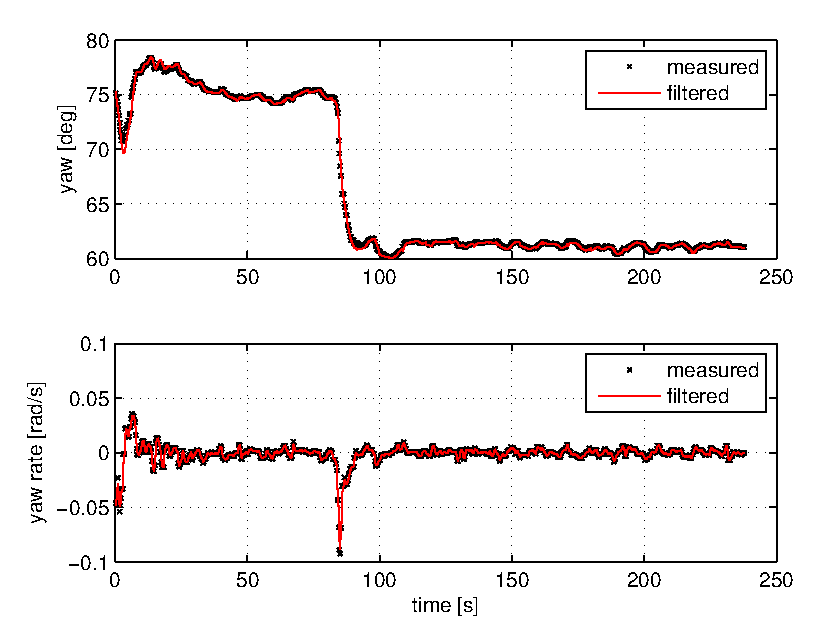
\includegraphics[width=0.48\linewidth]{simulations/fig/yaw-straight2.eps}} \\   
\caption{AUV localisation using EKF with high confidence in yaw measurement, SDyaw = 0.01$rad \approx 0.6 ^{\circ}$. SDyawRate = 0.004 $\frac{rad}{s}$, SDu/v = $1\frac{cm}{s}$.}

\label{fig:auv-sim-straight2}
\end{figure}
\begin{figure}%[htb]
  \centering
    \subfigure[N/E localisation. Yaw was calculated by integrating yaw rate periodically measured using FOG.] {\label{fig:sim-straight1}
	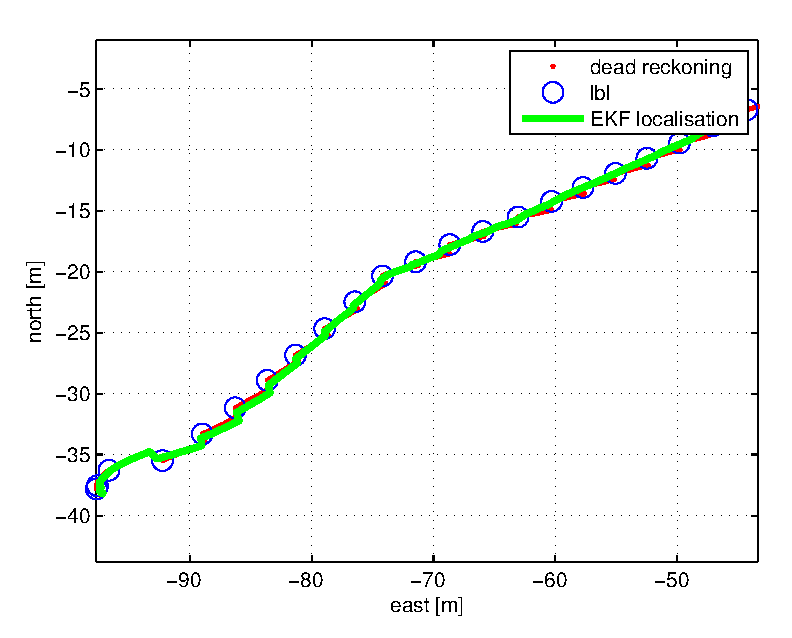
\includegraphics[width=0.48\linewidth]{simulations/fig/sim-straight1.eps}}
    \subfigure[Heading estimation. Biased yaw measurement is being corrected.] {\label{fig:yaw-straight1}
    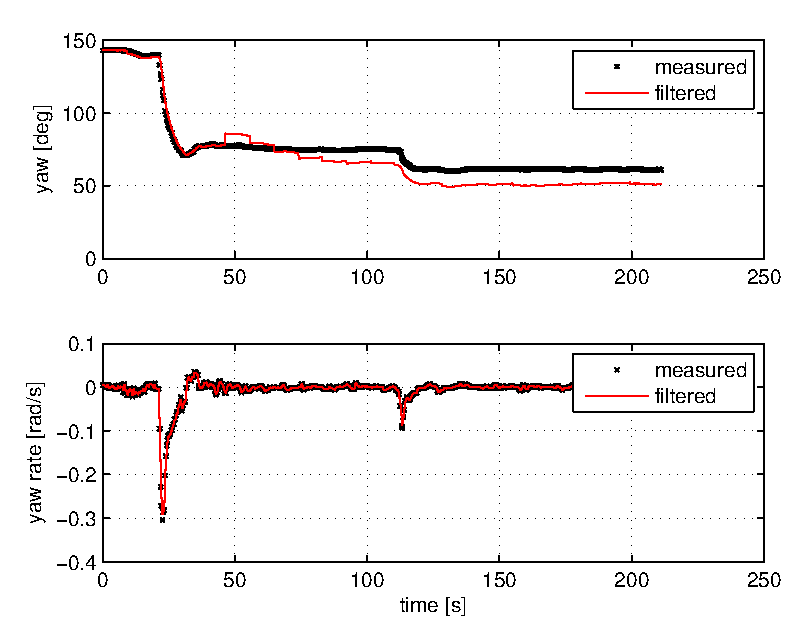
\includegraphics[width=0.48\linewidth]{simulations/fig/yaw-straight1.eps}} \\
\caption{AUV localisation using EKF with low confidence in yaw measurement, SDyaw = 0.2$rad \approx 11.5 ^{\circ}$. SDyawRate = 0.004 $\frac{rad}{s}$, SDu/v = $1\frac{cm}{s}$.}
%\vspace{-10pt}
\label{fig:auv-sim-straight1}
\end{figure}    
%After  initial heading, yaw rate was integrated in time to calculate yaw.    when setting  EKF parameter uncertainty  when using EKF, this time
EKF updates periodically (synchronous mode), with period set to 230 ms. At first, simulation parameters \textit{SDnorth}, \textit{SDeast}, \textit{SDyaw} and \textit{SDyawRate} were set to low values - suggesting high trust in measurements. Resulting trajectory (Figure ~\ref{fig:sim-straight2}) shows that the heading measurement has a constant bias, caused by the error in initial heading measurement obtained by compass. Thus, yaw measurement, calculated relative to previous value each time, propagates the error (bias). Biased yaw observation further on causes EKF localisation to experience sharp jumps. To overcome this using EKF framework, less confidence was assigned to the yaw measurement (\textit{SDyaw}) value. Eventually, bias becomes visible if measured and filtered heading are compared (Figure ~\ref{fig:yaw-straight1}). As for the rest of the heading information, rate of yaw measurement will be incorporated with a lot of confidence (\textit{SDyawRate} parameter having range of degrees) since it is a reliable device and it does not depend on the initial estimate. Good feature of sensor fusion is that lack of one measurement or its low performance can be compensated with some other measurement considering that they are combined together in mathematical model in the right manner. In case of yaw and yaw rate - the derivation in time is a relation that connects them together. 

Simulation shows that localisation performance can be tailored by setting the confidence in prediction model or measurement values. Confidence is materialized as standard deviation (variance) of the random variable: the lower it is, more certain the value of the random variable is hence more confident in value of that variable we tend to be. Kalman filter tries to optimise the result within the defined boundaries of uncertainty. 

Unscented Kalman filter was mentioned in Section \S~\ref{sec:ukf} as a good alternative in handling nonlinearities. UKF was implemented in MATLAB for the simulation purposes and its result compared with the EKF localisation, under same parameter settings and using the real data obtained from Nessie sensors. Test mission consisted of pipe tracking where the vehicle was guided along the underwater pipe three times and each time returned back to the initial position (Figure ~\ref{fig:ekf-ukf}). 2D north-east maps were compared, together with dead reckoning, same as one used for previous simulations. General characteristics of UKF are visible from the obtained shape of the UKF path (Figure ~\ref{fig:ekf-ukf}). Eventually, both filtered paths end up in approximately same position, having less drift than the dead reckoning. EKF does first order approximations, therefore, its path is slightly distorted compared with the UKF one, which was obtained with the same amount of calculation, and the inherited approximation of at least second order \cite{julier96}. Simultaneously with filtering, UKF preserves the nonlinearity formula of prediction model better - its curves have shape closer to equation-based dead reckoning curves. Still, a question that is yet opened is whether we need to improve the approximation of the prediction model. Answering this question is a hard task without knowing the movement of the object and how much it actually matches the state prediction model. A difficulty with UKF implementation is that it involves calculation of covariance matrix square root which is a slightly more complex problem, solved with numerical methods. Nevertheless, it is possible that covariance matrix becomes singular which also depends on parameter $k$ used for scaling (Section \S~\ref{sec:ukf}). $k$ was set to -0.5 for simulations shown.        
\begin{figure}%[htb]
  \centering
    \subfigure[N/E localisation. Comparison of the EKF and UKF.] {\label{fig:ekf-ukf}
	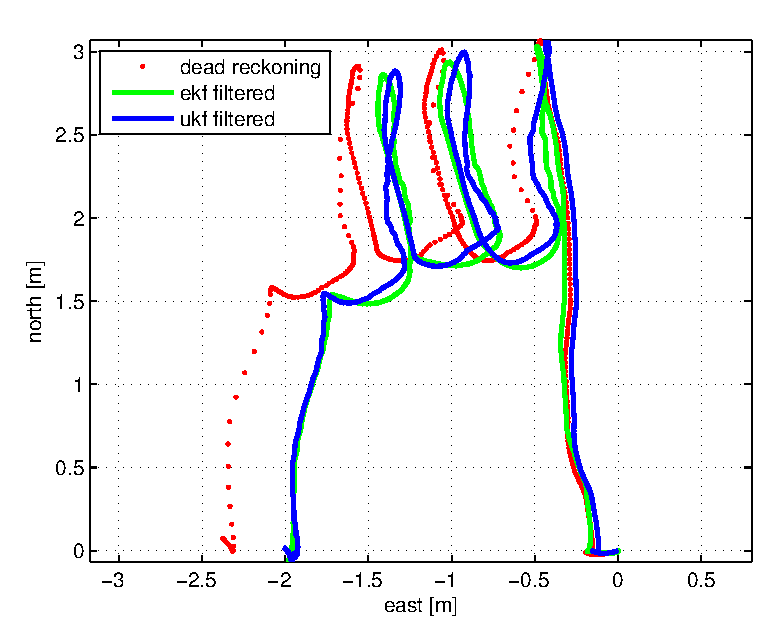
\includegraphics[width=0.42\linewidth]{simulations/fig/UKFpipeTrack.eps}}
    \subfigure[Magnetic disturbances affecting the heading measurement by compass. Vehicle is not moving, FOG is not oscillating at the same time.] {\label{fig:magnetic-disturb}
    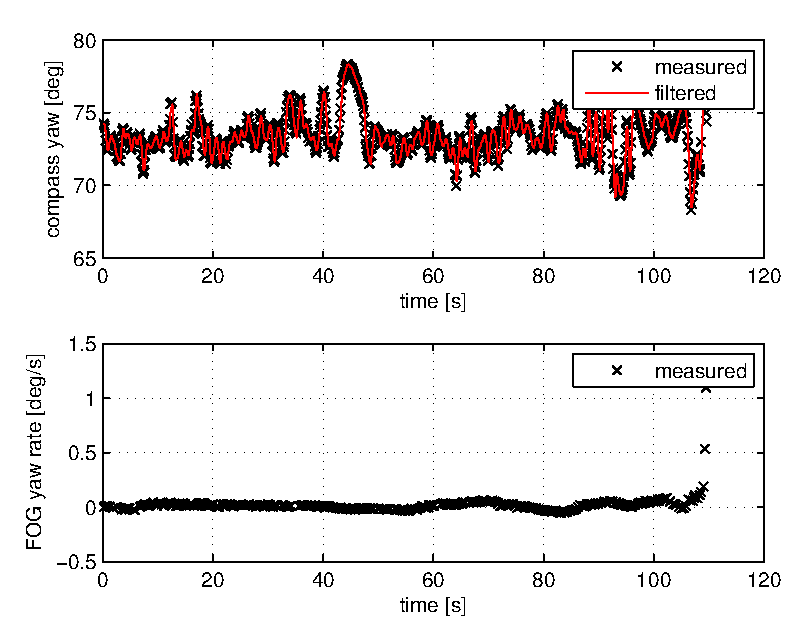
\includegraphics[width=0.42\linewidth]{simulations/fig/magnetic.eps}} 
%\vspace{-33pt}  
\end{figure}

\T{Sensor fusion for heading: } being in search for heading measurement less prone to initial error, and guided by simulation results, real scenarios were accomplished using magnetic compass for heading measurement. Compass is more sensitive to magnetic disturbances (Figure ~\ref{fig:magnetic-disturb}), slower than FOG but, importantly, gives an absolute measure. Therefore, it does not rely on previous measurements. An experiment was made by just manually rotating the robot horizontally while keeping the same position - changing its heading. Figures ~\ref{fig:lostFog} and ~\ref{fig:lostCompass} show the performance of yaw filtering using EKF and the example of sensor fusion of compass and FOG. Namely, compass (Figure ~\ref{fig:lostCompass}) or FOG (Figure ~\ref{fig:lostFog}) were disabled at one point during the experiment. When one of them stops working, the other one tries to compensate the failure. 
%and still filters the heading/yaw rate variation.  
\begin{figure}%[htb]
  \centering
    \subfigure[Compass disabled.] {\label{fig:lostCompass}
	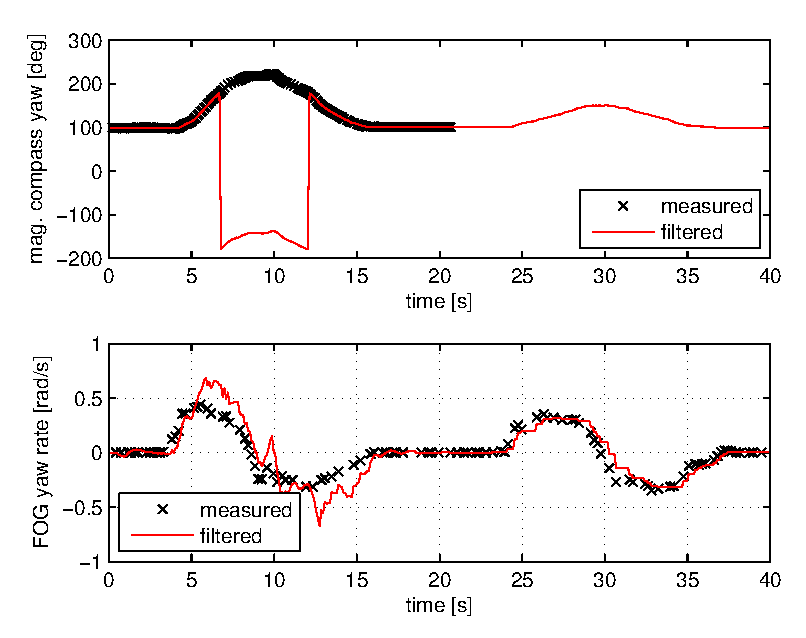
\includegraphics[width=0.45\linewidth]{results/fig/lostCompass.eps}}
    \subfigure[FOG disabled.] {\label{fig:lostFog}
    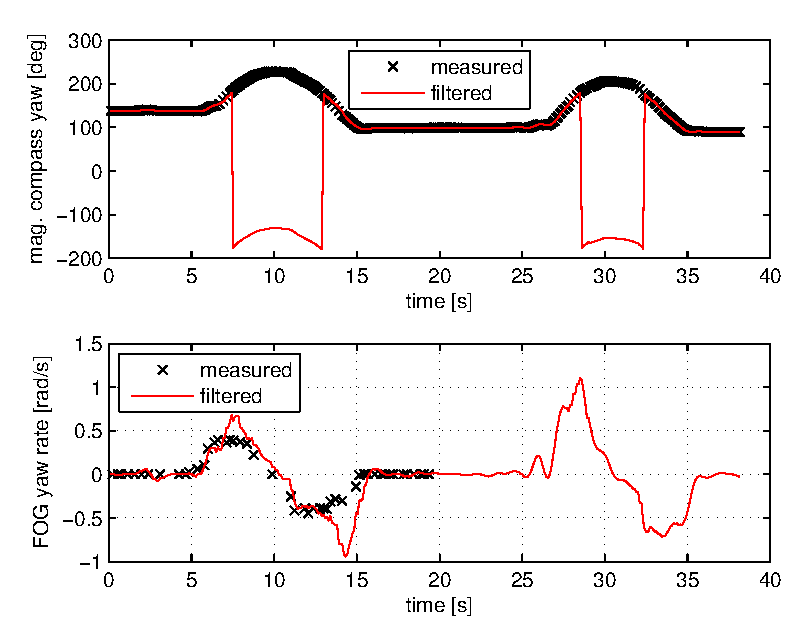
\includegraphics[width=0.45\linewidth]{results/fig/lostFOG.eps}} \\   
\end{figure}

\T{Trajectory filtering: } Spiral trajectory and surfacing action was taken with Nessie starting from the depth of around 12 m. EKF filtering results are shown in Figure ~\ref{fig:spiral} together with LBL position updates and dead reckoning starting from each position. Similarly as with previous plots, dead reckoning was shown together with LBL position updates. Filtered trajectory does not experience severe jumps, and the curve seems to be smoother and less prone to drifting. Standard deviation of north and east measurement parameter (Table ~\ref{tab:ekf-params}) was tested with different values, causing more or less confidence in LBL measurement hence shaping the filtered localisation curve. Presented LBL measurements are exhibiting quite diverse range of values.

Causes of position correction errors are numerous: from ``multipathing'' outliers (Figure ~\ref{fig:multipathing}) till the imprecision inferred from the nature of volatile acoustic and GPS information. ``Multipathing'' causes outliers in position information as a result of false reflections for instance. Acoustic and GPS imprecision can be treated as Gaussian random variable. 
\begin{wrapfigure}{r}{0.55\textwidth}
\vspace{-10pt}
  \centering
    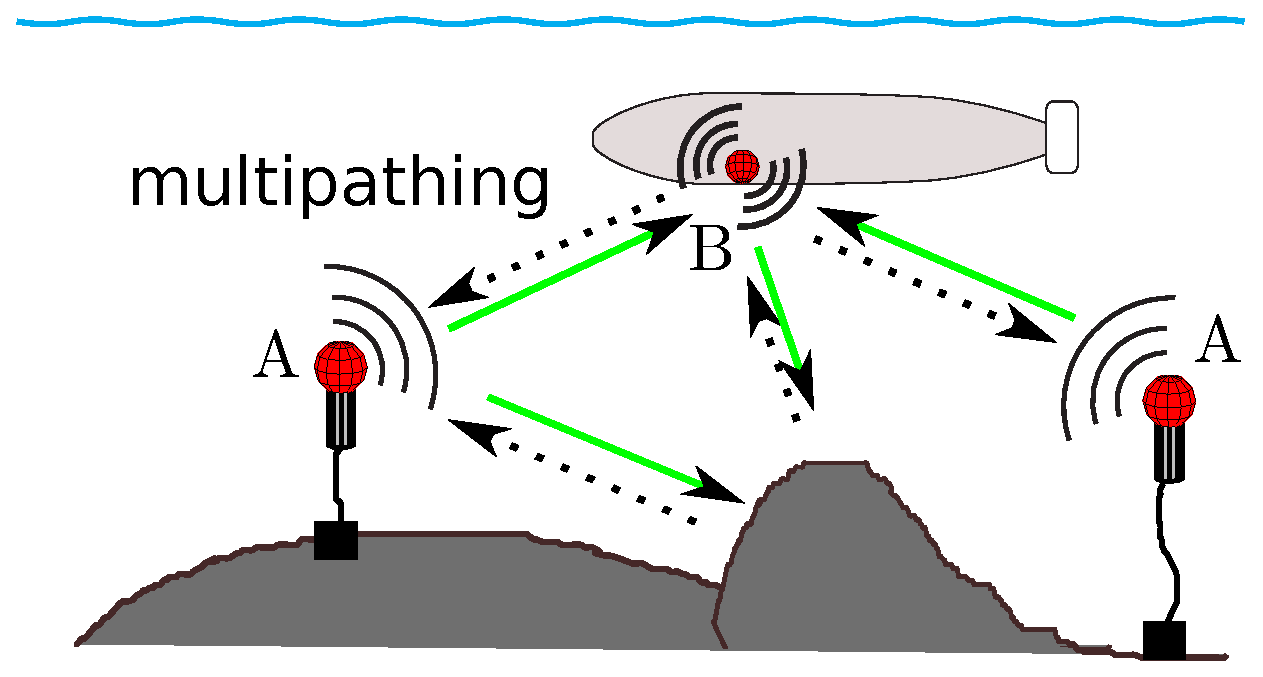
\includegraphics[width=0.45\textwidth]{results/fig/multipathing.eps}
  \caption{Multipathing can cause outliers in LBL position measurement. Due to reflection, several distances are detected, some  being false measurements.}
%\vspace{-10pt} 
\label{fig:multipathing}
\end{wrapfigure}
It is likely that some of the LBL position updates deviate from the trajectory. Hence, a mechanism for rejecting the outliers was investigated. EKF was tested on raw LBL position updates. Intention is to manage the filtration of the ``outliers'' by using properly tuned EKF. Motivation to explore such possibility comes from two scenarios encountered in earlier missions. In such missions position wad dead reckoned and LBL was used to assign each time a new value of north and east coordinate. LBL outliers were ruled out using a median filter applied on the last eleven position coordinates once the latest LBL exceeded the set threshold in position change. The missions showcased situations when: 
\begin{itemize}
\item LBL rejection is carried out despite being a ``false alarm'' - Figure ~\ref{fig:straight-median-ekf},
\item rejection of the LBL is the right choice - Figure ~\ref{fig:spiral-median-ekf}
\end{itemize}
It is important to say that LBL position filtering was implemented in form of median filter. EKF was updated with raw LBL data instead of median filter. Rejecting an LBL measurement can turn out to be right (Figure ~\ref{fig:spiral-median-ekf}) as well as a wrong decision (Figure ~\ref{fig:straight-median-ekf}). That is why EKF was suggested as an alternative. Examples of EKF's performance are shown in both Figures ~\ref{fig:straight-median-ekf} and ~\ref{fig:spiral-median-ekf}. Solution is not as categoric as median filter. Moreover, it is more robust. By giving certain trust in LBL observation it always takes it into account. Median filter, on the other hand, can be too selective in being right or wrong. If it turns out that LBL positions do follow each other, EKF continues slowly following that direction. If the outliers are isolated, EKF successfully rules them out (Figure ~\ref{fig:spiral-median-ekf}). 
\begin{figure}%[htb]
  \centering
    \subfigure[Straight trajectory: LBL outliers erroneously rejected (red). EKF tends to recover the navigation (green).] {\label{fig:straight-median-ekf}
	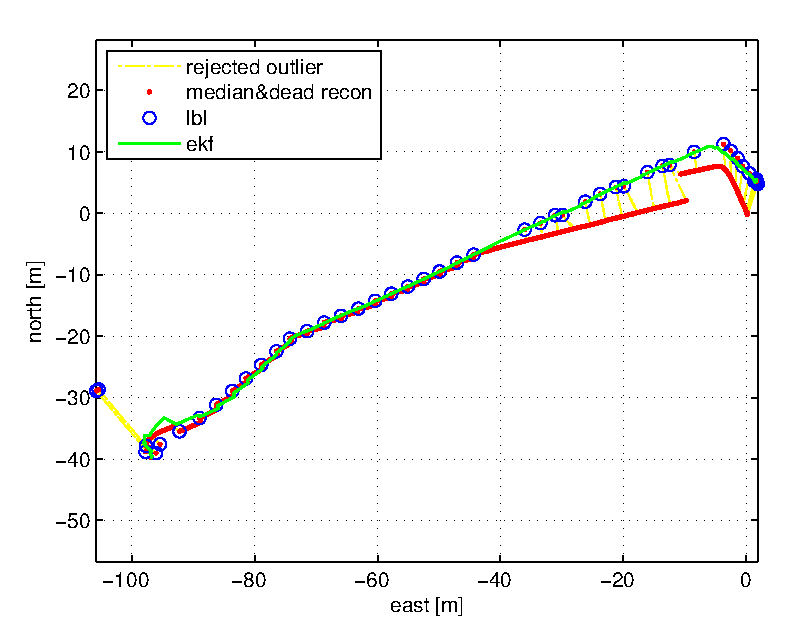
\includegraphics[width=0.47\linewidth]{results/fig/straight-median-ekf.eps}}
    %\subfigure[Straight trajectory: LBL outliers filtered with EKF.] {\label{fig:straight-ekf}
    %\includegraphics[width=0.45\linewidth]{results/fig/straight-ekf.eps}} \\  
    \subfigure[Spiral trajectory: LBL outliers are rejected using median. EKF filtering introduces the position disturbance which recovers soon after.] {\label{fig:spiral-median-ekf}
    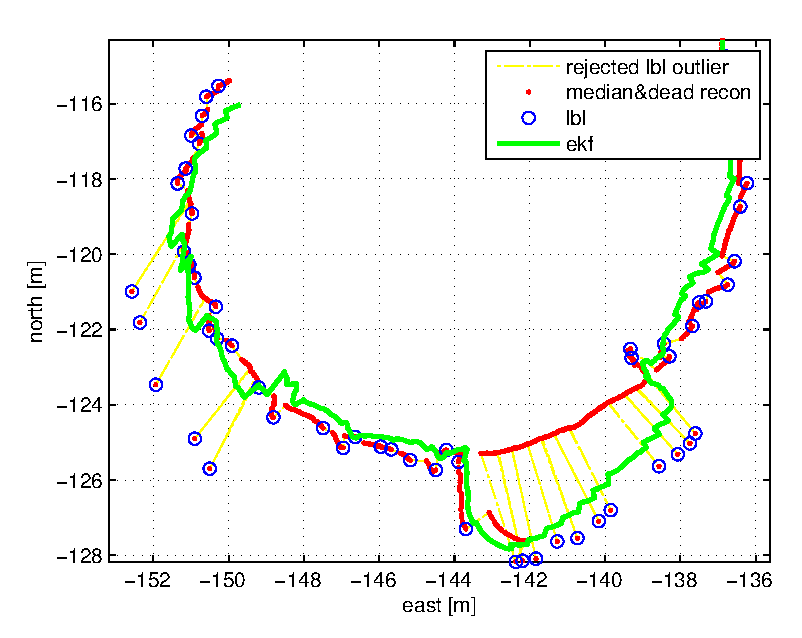
\includegraphics[width=0.5\linewidth]{results/fig/spiral-median-ekf.eps}} 
    %\subfigure[Spiral trajectory: LBL outliers filtered with EKF.] {\label{fig:spiral-ekf}
    %\includegraphics[width=0.45\linewidth]{results/fig/spiral-ekf.eps}}     
\end{figure}

\T{Square trajectories: } square trajectories were tested in low depths of a lake, with the GPS signal available to be used as a position reference and ground truth indication (Figures ~\ref{fig:no-gps}, ~\ref{fig:with-gps}). Dead reckoning navigation was used as a reference when controlling the vehicle movement during the experiment. This fact can cause slight confusion in analysis of the trajectory graphs since all the dynamics and forces were applied with respect to the dead reckoning navigation which is an estimated value, not the real existing one. It is a slightly inverse logic of testing, nevertheless further tests are yet to be accomplished. Emphasis of this experiment was to show that EKF can work successfully and analyse the main characteristics of the navigation design. It is likely that the GPS emulated square-shaped trajectories float as the elapsed path becomes longer. GPS signal available from the antenna located on the water surface is serving as a measure of absolute position within the lake - giving an idea about the actual vehicle position while it tries to moves within the boundaries of estimated dead reckoning position. 

Main issue when performing the square trajectory tests was significant imprecision of GPS signal. Many reasons can possibly influence the imprecision: from the weather conditions till surrounding objects. Basically anything that can affect the satellite visibility and the quality of the signal. Drifting can reach up to several meters which is unacceptable considering the trajectory length. Finally, the trajectory of the experiment itself is quite short ($ \approx 10 m $) to be seriously and accurately covered with precise GPS position update. Figure ~\ref{fig:gps} shows the tested trajectory and depicts the encountered amount of GPS imprecision.
\begin{figure}%[htb]
  \centering
    \subfigure[Coordinates of the tested square trajectory pasted on the lake map.] {\label{fig:gps-map}
	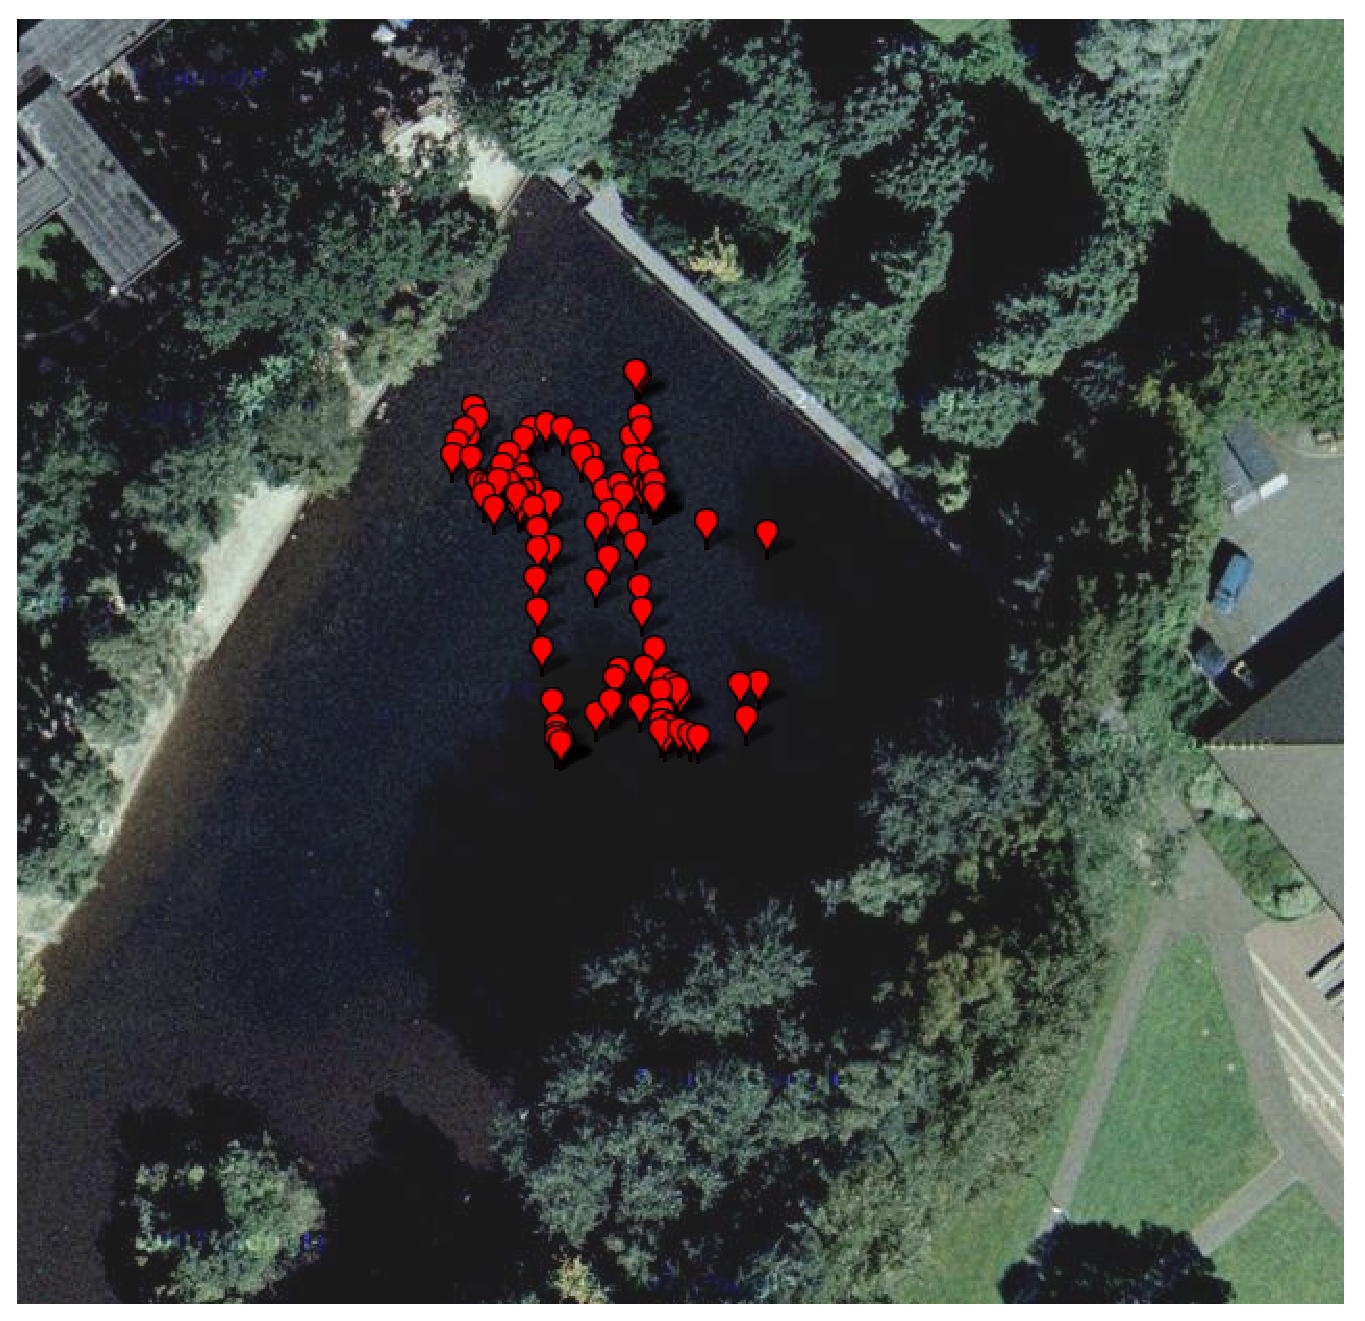
\includegraphics[width=0.48\linewidth]{results/fig/square-trajectory.eps}}
    \subfigure[GPS signal as it appears originally.] {\label{fig:gps-signal}
	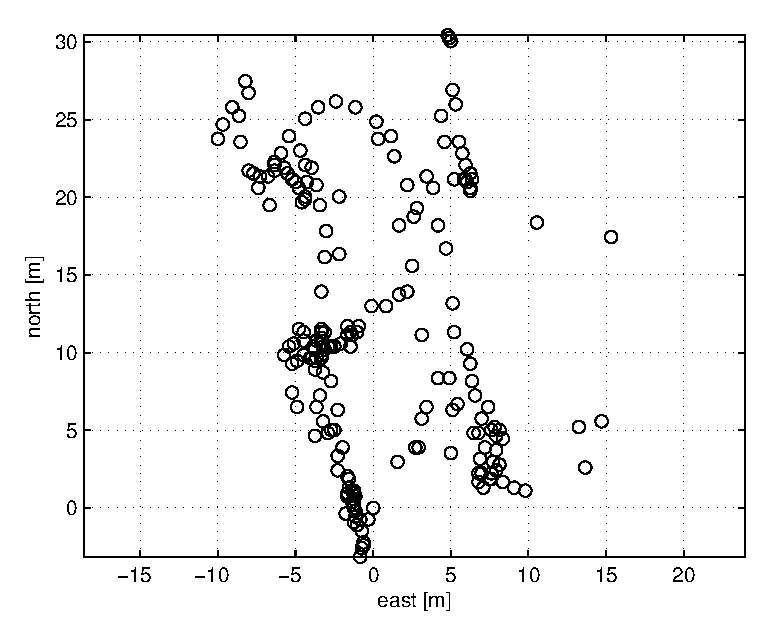
\includegraphics[width=0.48\linewidth]{results/fig/gps-signal.eps}}
\end{figure}

\T{Without GPS: } EKF localisation was tested in given conditions. Initially, only motion (inertial) sensors were used within the observations. That implies all the available linear and angular velocity sensors. Absolute position (raw GPS signal in this constellation) was not included in observations. EKF periodically updates (synchronous mode, \S~\ref{chap:methodology}), with the rate of 10 Hz. The aim was to measure the performance and the amount of drifting that occurs since the robot is intended to repeatedly attain square-like paths and return to the starting position in ideal scenario. It is useful to mention that proper parameter tuning can significantly change filtering performance. By giving more or less trust in particular measurement, or particular model behaviour, the role of certain parameters of dynamics (velocities, angular velocities) can be emphasized if necessary. Figure ~\ref{fig:no-gps} shows the performance of EKF without GPS position correction after one trajectory cycle, and the original path that was followed, recorded using GPS. Initial position was taken from the first GPS measurement and the first measurement can indeed be away from the real position due to GPS imprecision. Note that the control of the vehicle trajectory refers to dead-reckoning calculated north-east values, not some physical beacons with known position. At the time of reporting the experiments, testing were not fully completed with all the planned scenario variations. Localisation expectedly tends to perform with a significant drift without the absolute position update (Figure ~\ref{fig:square-1-noGps}). After the second square-shaped cycle (Figure ~\ref{fig:square-2-noGps}), EKF shows that it roughly tracks the shape of the trajectory, smooths it by filtering out the measurement outliers. Vehicle has returned approximately to the same position after each cycle. Drift gained when following one of the sides of the rectangular path was compensated with the same amount of drift but of the opposite sign that was active when taking the return direction. Enormous amount of drift is present since the information on absolute position is not considered. The first available GPS coordinate fixes the starting position and part of the initial position error is caused by being incapable of setting the initial position accurately.       
\begin{figure}%[htb]
  \centering
    \subfigure[N/E localisation.] {\label{fig:spiral2d}
	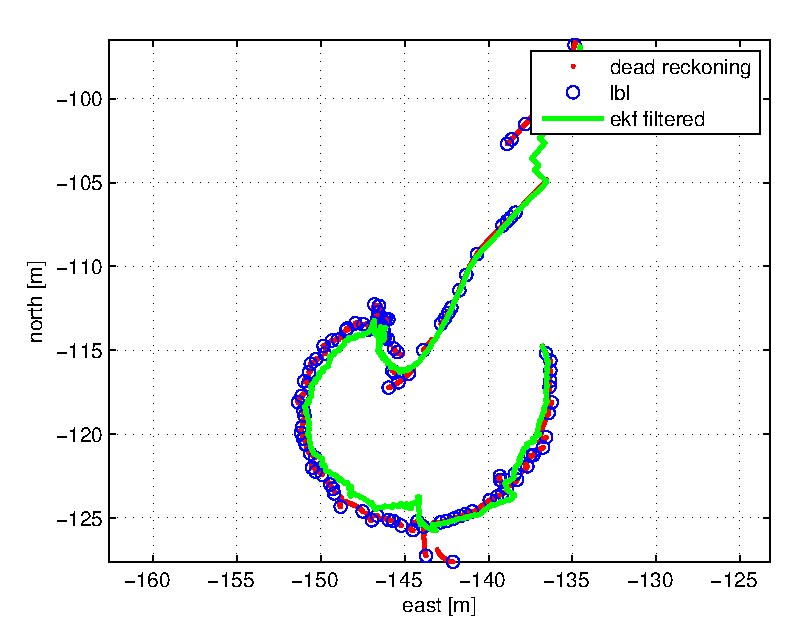
\includegraphics[width=0.48\linewidth]{results/fig/spiral2d.eps}}
    \subfigure[Depth.] {\label{fig:spiral-depth}
    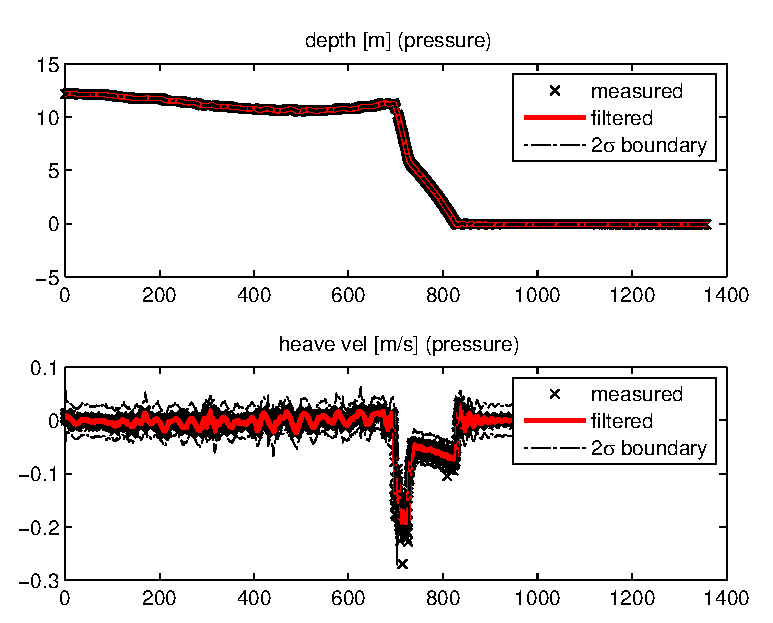
\includegraphics[width=0.48\linewidth]{results/fig/spiral-depth.eps}}
    % \\  
    %\subfigure[Path (temporary plot).] {\label{fig:spiral3d}
    %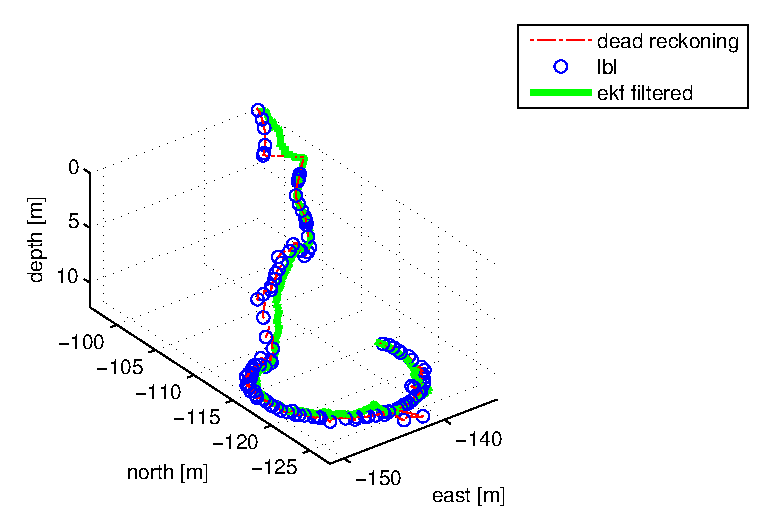
\includegraphics[width=0.8\linewidth]{results/fig/spiral3d.eps}} 
\end{figure}
\begin{figure}%[h]
  \centering
    \subfigure[EKF localisation after one cycle.] {\label{fig:square-1-noGps}
	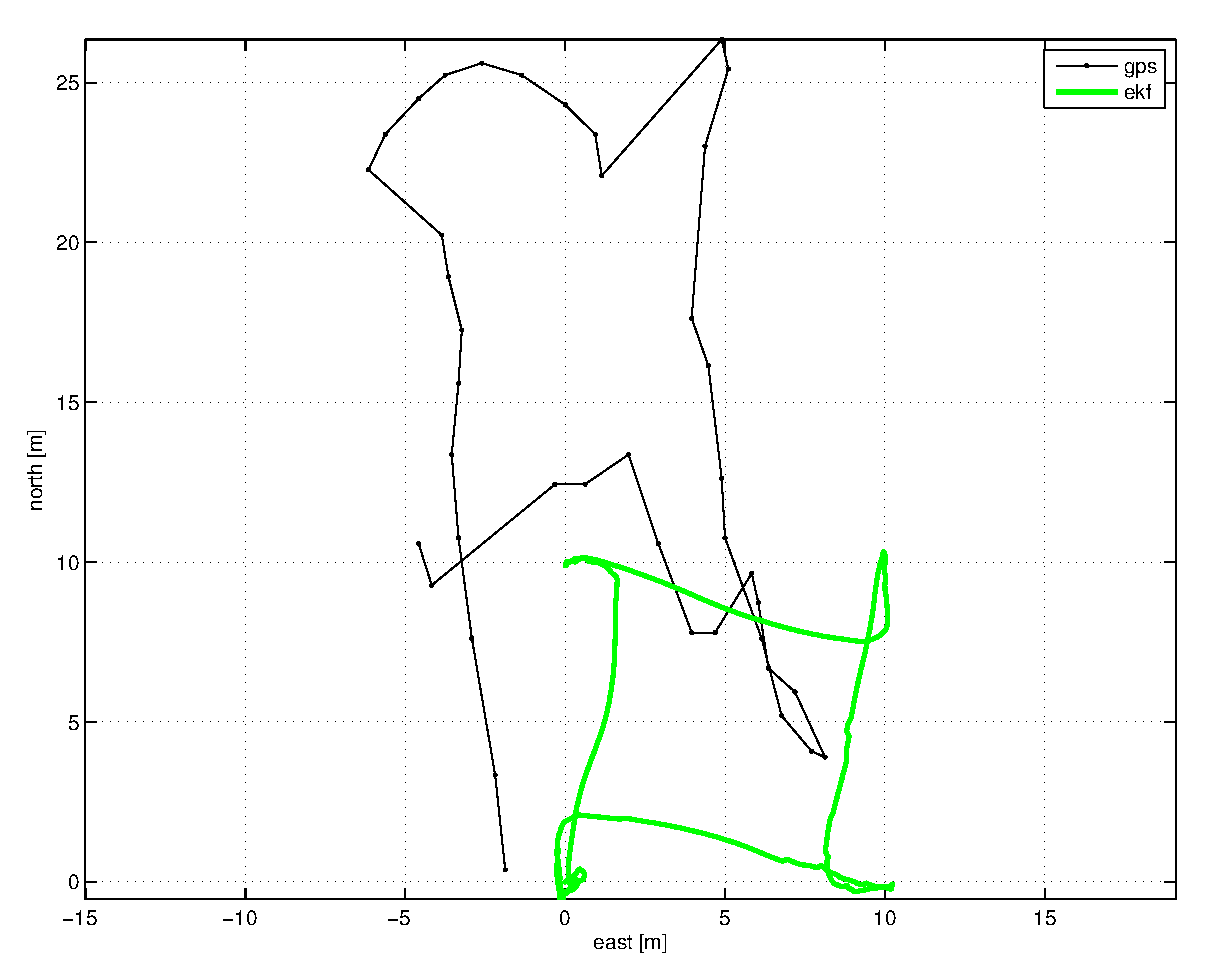
\includegraphics[width=0.48\linewidth]{results/fig/square1NoGps.eps}}
    \subfigure[EKF localisation after two cycles.] {\label{fig:square-2-noGps}
	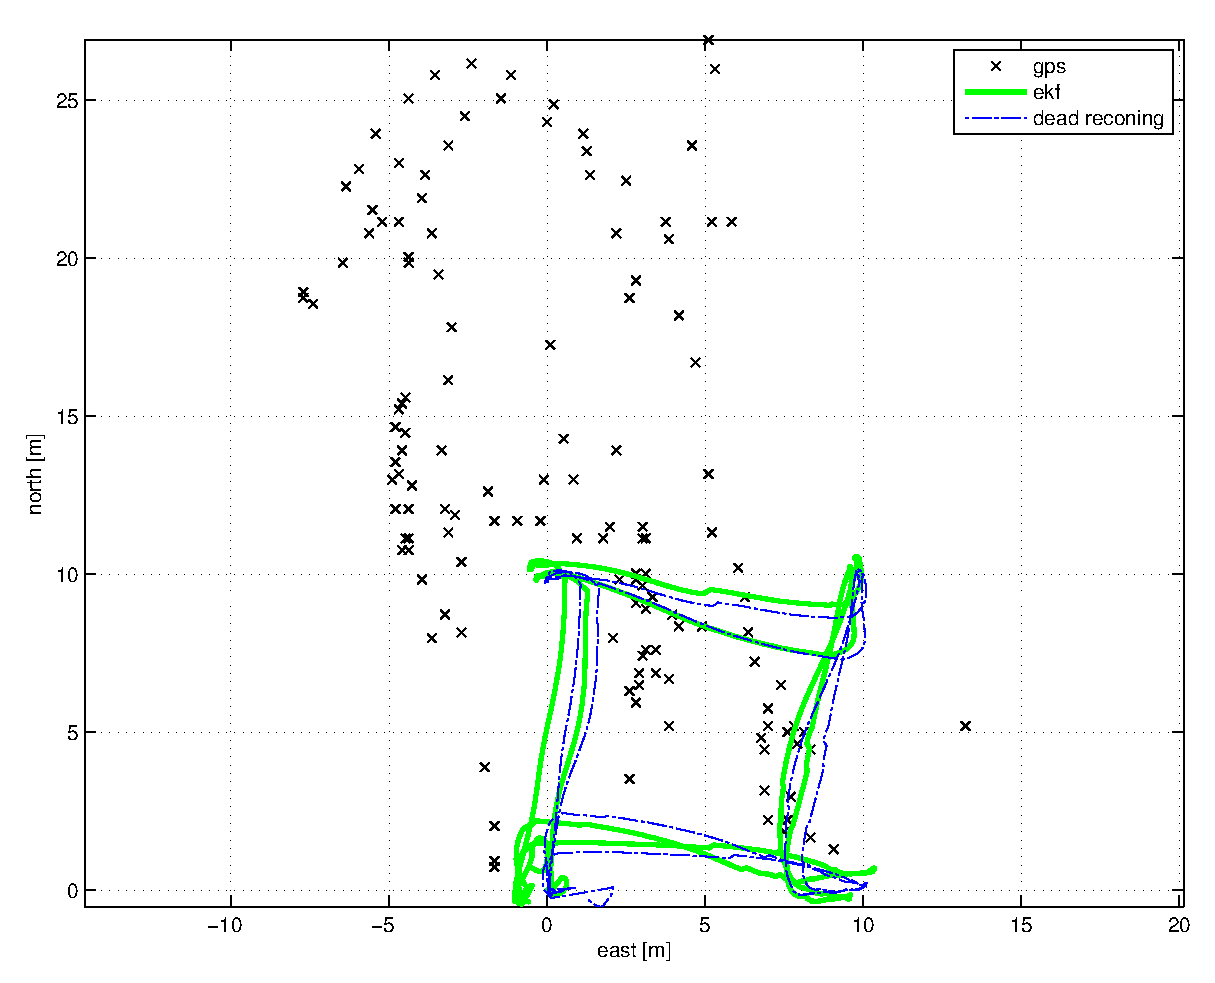
\includegraphics[width=0.48\linewidth]{results/fig/square2NoGps.eps}}\\
    %\subfigure[] {}
    %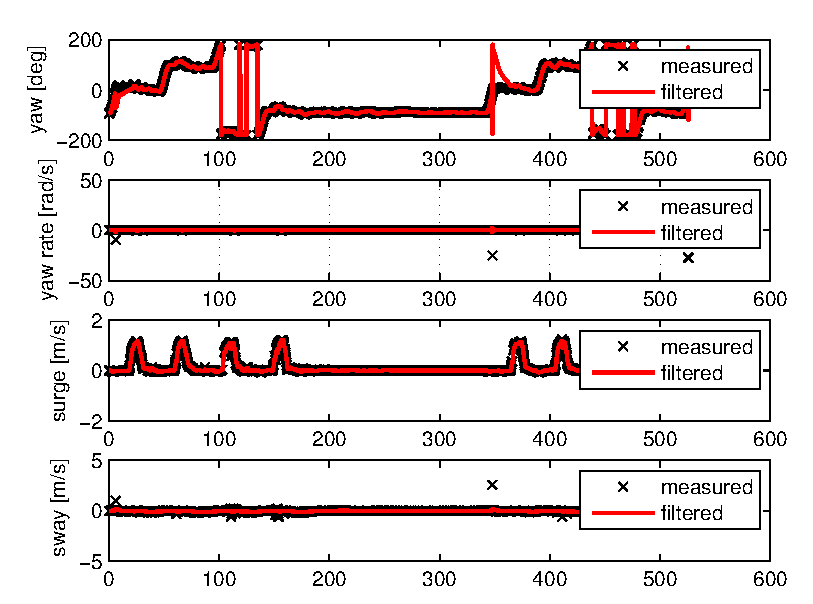
\includegraphics[width=0.6\linewidth]{results/fig/dynamics.eps}}
    \caption{EKF localisation using only inertial measurements as observation.}
    \label{fig:no-gps}
\end{figure}

\begin{figure}%[hb]%tb
  \centering
    \subfigure[Setting standard deviation of 1 m in uncertainty position observation (SDnorth = SDeast = 1.0 m).] {\label{fig:square-withGps-1}
	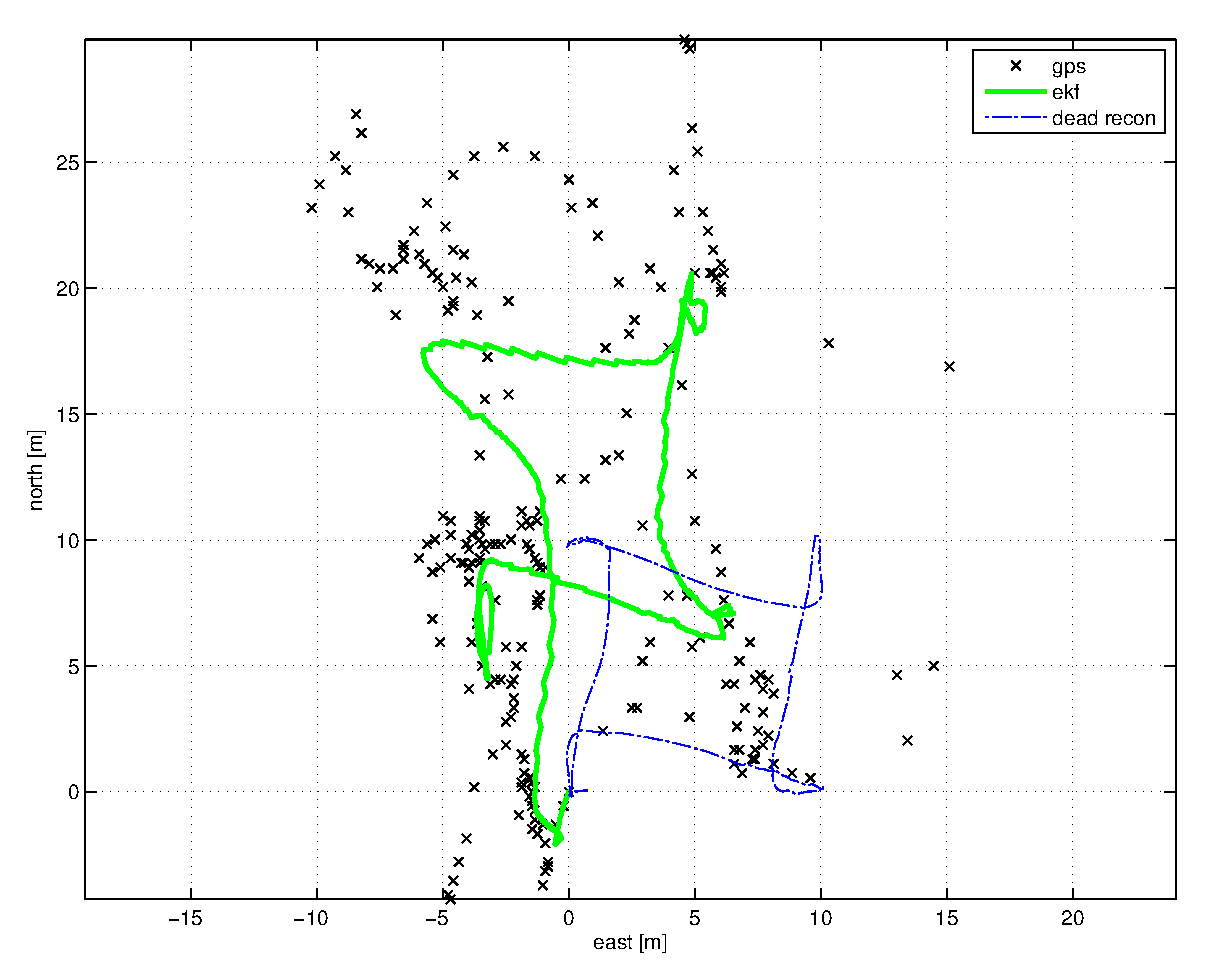
\includegraphics[width=0.48\linewidth]{results/fig/squareWithGps-10.eps}}
    \subfigure[EKF localisation after tuning the position uncertainty (SDnorth = SDeast = 0.5 m).] {\label{fig:square-withGps-2}
	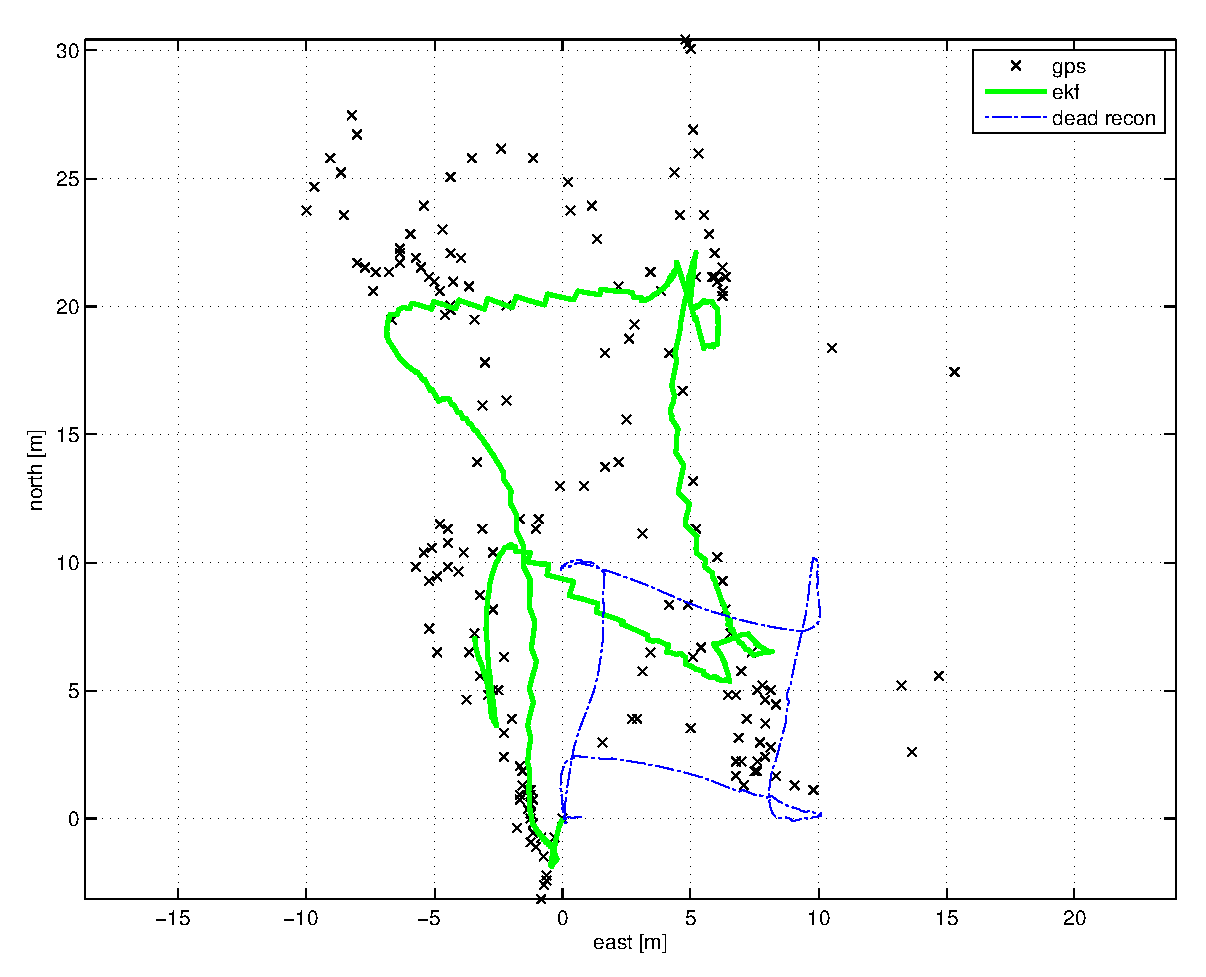
\includegraphics[width=0.48\linewidth]{results/fig/squareWithGps-05.eps}}
    %\\
    %\subfigure[Linear and angular velocities during square-shaped trajectory.] {\label{fig:square-dynamics}
    %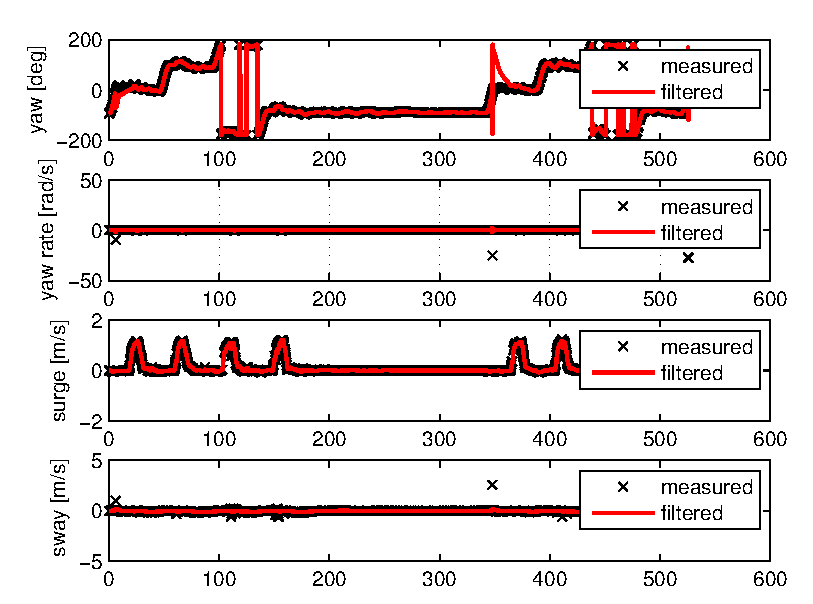
\includegraphics[width=0.45\linewidth]{results/fig/dynamics.eps}}
    \caption{EKF localisation aided with GPS position updates weighted by setting appropriate parameters.}
    \label{fig:with-gps}
\end{figure}
\begin{figure}
\centering
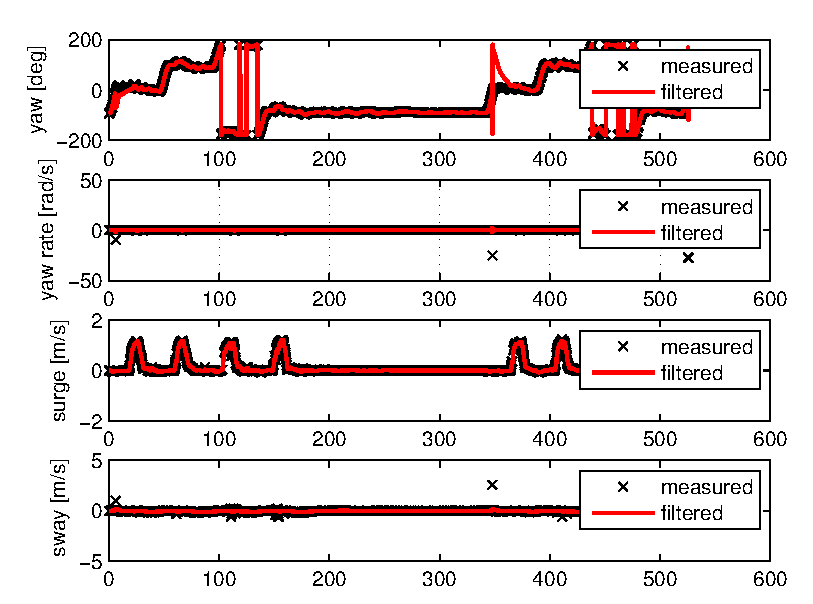
\includegraphics[width=0.6\linewidth]{results/fig/dynamics.eps}
\caption{Linear and angular velocities during square-shaped trajectory.}
\label{fig:square-dynamics}
\end{figure}
\T{With GPS: } Finally, GPS measurements were appended to the EKF observations. Localisation results were shown in Figure ~\ref{fig:with-gps} for two different level of confidence (variances) in position measurement. Naturally, giving extremely high confidence does not seem to be the best choice, however, some empirically deduced values in range of decimetres significantly correct the dead reckoning drift. Furthermore, EKF tends to filter the GPS measured north east coordinates, hence partially corrects the GPS imprecisions stated at the beginning. At this point it is evident why EKF is a great tool. Filter tries to satisfy the set uncertainty boundaries and fuse all the available information trying to make the most out of it combined together in one mathematical system. Moreover, fusing such imprecise and sketchy position data from GPS, still improves the localisation. Obtained trajectory tends to go towards what can be treated as expected path. From something that looked like a noisy collection of position observations at the beginning (Figure ~\ref{fig:gps-signal}), application of EKF together with sensor fusion enabled having generally better performance in navigation.     
%Combination of all relevant sensors gives in a Kalman filter state estimate results in more precise position and heading compared with instant (flat) usage of position and orientation measurements.  
%\subsection{Sensor selection}
%Design and performance test.
%\subsection{Using FOG for navigation improvement}
%How big is the improvement with respect to the distance travelled?
